\chapter{Mise en oeuvre des concepts dans l'environnement \texttt{Cast3M}}
%~\footnote{Annexe rédigé par A.Constantinescu (LMS - CNRS - Ecole Polytechnique, 91128
%Palaiseau cedex, France)}

\section{Historique}

Le Commisariat à l'énérgie atomique (CEA, Saclay, France) a développé depuis une vingtaine 
d'annéés une boite à outils: \texttt{Cast3M}, incorporant les éléments nécessaires pour ménéer à bien 
une analyse en utilisant la méthode des éléments-finis. Son champs d'aplication privilégie 
la mécanique (élasticité, élastoplasticite, \ldots) mais également la thermique, l'hydraulique 
ou l'éléctromagnetisme. Il est important de souligner, que son caractère modulaire permet facilement 
de traiter des problèmes couplés ou encore multiphysique. 

\texttt{Cast3M} est fondé sur une famille d'\textit{objets}, i.e. 
structures des données et sur un lexicon d'\textit{opérateurs}, i.e. opérations élémentaires 
agissant sur les objets, le deux formant un langage propre de programmation appelé \textsc{gibiane}. 
Cette possibilité de programmation directe le différencie par 
rapport aux codes classiques qui sont généralement 
dédiés à des opérations spécifiques. 

Sur le site: \texttt{http://www-cast3m.cea.fr/} on trouve une présentation générale du code, 
des fichiers d'exemples et des introductions à son utlisation, ainsi que les versions 
\texttt{windows} et \texttt{linux} du code. Le CEA met gracieusement \texttt{Cast3m} à la disposition 
des utilisateurs non-commerciaux. 

Dans cette annexe on se propose d'introduire les objets éléments finis de \texttt{Cast3M} et 
leur relation avec les concepts présentes dans le cours et de donner quelques examples. 

\section{Présentation générale}

Du point de vue programmation on différencie en \texttt{Cast3M} deux niveaux 
de programmation:
\begin{itemize}
\item \textit{un langage de bas niveau compilé}~: \textsc{esope}. Ce langage il est invisible pour l'utilisateur normal,
est le langage de prédilection des créteurs de \texttt{Cast3M}. Il n'est qu'un dérivée de \textsc{Fortran} auquel on a
rajouté des opérations pour la manipulation des objets spécifiques;
\item \textit{un langage de haut niveau interpreté}~: \textsc{gibiane}, formé d'un lexicon des opérations 
sur les objets et qui permet une utilisation facile du code et qui est le langage de l'utilisateur normal. 
\end{itemize}
De ce point de vue, \texttt{Cast3M} est comparable à des code du type \texttt{Mathematica, Matlab, Scilab, \ldots},
\textsc{esope} étant le langage privilégie du créateur du code et \textsc{gibiane} étant le langage 
spécifique de l'utilisateur.  Dans la suite on va juste discuter de la programmation haut niveau 
en \textsc{gibiane}, qui reste transparente pour l'utilisateur.   

L'utilisation du langage \textsc{gibiane}~\footnote{La pluspart des noms d'opérateurs provient du 
noms commun en français désignant l'opération. Cependant une version anglaise 
des opérateurs est également disponible.} 
peut être résumé ainsi~: \\
\centerline{\texttt{ objet\_2 = opérateur objet\_1 ; }}
Le signe ";" obligé le  système d'exectuter l'\texttt{opérateur} ayant comme donnée l'objet 
\texttt{objet\_1} et de créer un nouveau objet résultat \texttt{object\_2}. Avant de 
continuer on précise quelque régles de syntaxe en \textsc{gibiane}:
\begin{itemize}
 
 \item les noms des opérateurs se distinguent par leur premières quatres charactères, ainsi
 \texttt{vibr} désigne l'opérateur  \texttt{vibr[ation]}.
   
 \item les noms des objets ne doivent pas dépasser 8 lettres.
 
 \item les lignes ne doivent pas dépasser 72 charactères.
 
 \item le code n'est pas capable de faire la distinction entre lettres minuscules
 et majuscules, donc \texttt{vibr} est équivalent à \texttt{Vibr} ou 
 encore \texttt{VIBR}.      

\end{itemize}
Les objets sont des données numériques, logiques décrivant des object mathématiques 
ou physiques. On retrouve les types d'objets classiques décrivant des nombres:
\texttt{entier, flottant, logique} (en anglais \texttt{integer, real, logical}), 
et une série d'objets typiques pour un calcul par éléments fini, par exemple~:
\begin{itemize}

\item le \texttt{maillage} et décrit par un type d'élement, une liste 
des \texttt{noeuds} et leur connectivité;

\item un \texttt{chpoint} (champ par point) représent a un champ défini sur un domaine 
décrit par un maillage et ses valeurs aux noeuds, comme la temperature, le déplacement, \ldots;

\item le \texttt{mchaml} (champs par élément) représent a un champ défini sur un domaine 
décrit par un maillage et un type d'élémént fini ainsi que ses valeurs aux 
points spécifiques comme par exemple les points d'intégration de Gauss. Des exemples 
des champs représentés en utilisant des champs par points sont 
les contraintes, les déformations, le gradient de la temperature, \ldots;

\item la \texttt{rigidité} est un objet de type matrice de rigidité avec des eventuelles 
préconditionements.

\end{itemize}

Les opérateurs élémentaires sont développées pour résoudre une multitude des 
manipulations:
\begin{itemize}

\item \texttt{+, *, / , - , ** }, sont les opérateurs algébriques 
fondamentaux et s'applique en égale mesure sur des nombres et des 
champs définis aux noeuds \texttt{chpoint} ou sur les éléments 
\texttt{mchaml};

\item \texttt{droi[te],cerc[le]} et  \texttt{surf[ace], dall[er]} permettent de 
contruire des droites et des cercles et respectivement des surfaces à partir 
des points ou des contours spécifiés. 

\item \texttt{plus} permet la translation relative to a given vector and
applies both to a \texttt{mchaml} type object and a \texttt{geometry} type object ;

\item \texttt{reso[ut]} solves the algebraic equation $\bfm{K} \bfm{X} = \bfm{Y}$, où $\bfm{K}$ est 
une matrice simétrique positive définie de type \texttt{rigidité} et $\bfm{X}$ et $\bfm{Y}$ sont 
des champs définis aux noeuds. 
 
\item \texttt{vibr[ation]} résout l'équation aux valeurs et modes propres $\bfm{K} \bfm{X} = \lambda \bfm{X}$, 
où $\bfm{K}$  une matrice simétrique positive définie de type \texttt{rigidité};

\item \texttt{masq[ue]} permet de trier les valeurs d'un champ par points \texttt{chpoint} ou par 
élément \texttt{mchaml} par rapport à un critère défini par l'utilisateur.

\end{itemize}
D'autres opérateurs sont purement algorithmiques~: 
\begin{itemize}

\item \texttt{si, sino[n], finsi} définisent un contrôl et sont équivalents aux opérateurs \texttt{if,
else, endif} des langages classiques comme \textsc{C,Fortran,\ldots}~;

\item \texttt{repe[ter], fin} définisent une boucle et sont équivalents aux opérateurs \texttt{do,
enddo} des langages classiques comme \textsc{C,Fortran,\ldots}~;

\item \texttt{debpr[ocedure]} et \texttt{finp[roc]} définissent une procédure en 
\textsc{gibiane} l'équivalent de \texttt{subroutine} 
\texttt{end} des langages classiques comme \textsc{C,Fortran,\ldots}  ;

\end{itemize}
Parmi les opérateurs graphiques on distingué~:
\begin{itemize}

 \item \texttt{dess[iner]} qui permet de dessiner une courbe à partir d'une série des paires de nombres. 
  
 \item \texttt{trac[er]} qui permet des representer un maillage ou les isovaleurs d'un champs 
 défini sur un maillage. 
  
\end{itemize}
Dans la suite on va présenter quelques examples de programmation en \texttt{gibiane} pour montrer
l'application des opérateurs élémentaires dans la construction des algorithmes d'intégration 
numériques, bien que la pluspart des problèmes discutés dans la suite peuvent être intégrées 
en utilisant des opérateurs complexes déjà existants comme \texttt{pasapas, dyna[mique), \ldots}.   

\section{Calcul élastique}

\begin{figure}
\centerline{
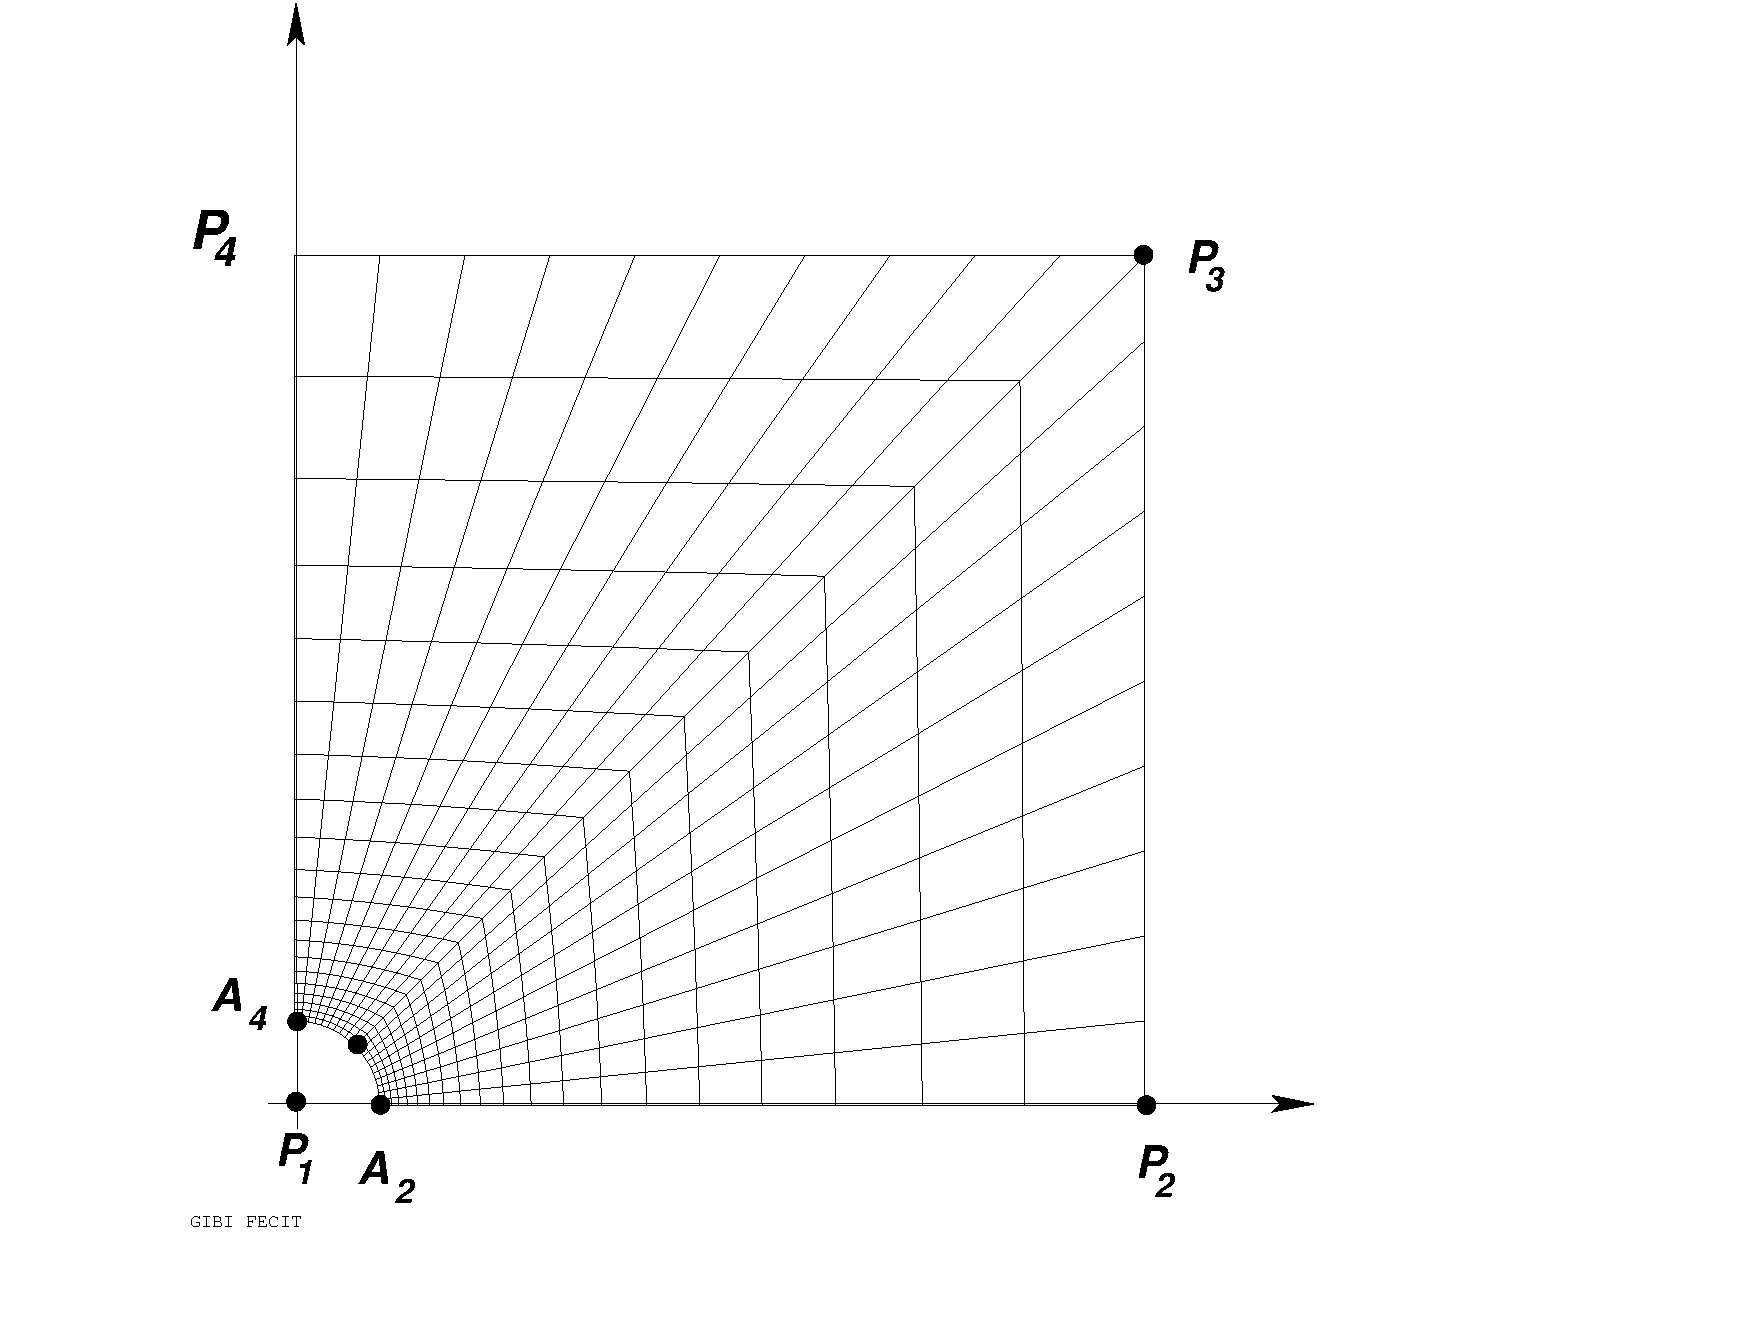
\includegraphics[height=5.cm]{./FIG/trou}
}
\caption{Le quart d'une plaque trouée en traction}
\label{fig:trou}
\end{figure}

\subsection*{Création du maillage}

\begin{castemcom}
L'opérateur \texttt{opti} ne crée pas des objets, mais défini les paramètres du calcul
en utilisant des mots clefs.  Une \texttt{dime[nsion]} 2 et par défaut une déformation 
plane par défaut ainsi que le choix d'un \texttt{élém[ent]} isoparamétrique 
linéaire dénommé \texttt{QUA4} en \texttt{gibiane}. 

Les points du maillage sont ensuite définies en fonction 
de la largeur du domaine \texttt{ldom} et du rayopn du trou \texttt{r}.     
(voir figure~\ref{fig:castem:trou})

\end{castemcom}
\begin{castemlines}
\begin{verbatim}
opti dime 2 echo 1 elem QUA4; 

ldom = 1.; r = 0.1; 

p1 = 0. 0.; 
p2 = ldom 0.; 
p3 = ldom ldom; 
p4 = 0. ldom; 

a2 = r 0.; 
a4 = 0. r; 
a3 = (r/1.4142) (r/1.4142); 
\end{verbatim}
\end{castemlines}

\begin{castemcom}
Les opérateurs \texttt{droit(e)} 
et \texttt{cerc[le)} permettent de construire les 
segments des droite du contour du maillage. Le 
nombre d'élements sur différents segments et donné par 
les paramètres \texttt{nelem} et 
\texttt{nel\_bis} ainsi que la dimension du prémier 
et du dernier élément précisé après le mots clefs 
\texttt{dini} et \texttt{dfin}. 

Le maillage \texttt{dom} et construit en utilisant 
l'opérateur \texttt{dall[er]} initialement en deux parties 
qui vont être regroupés en utilisant \texttt{et} ensuite.
L'utilisation  d'\texttt{inve[rser]} change le ordre de 
parcours des noeuds dans le contour pour obtenir 
le maillage correct. 

Et finalment le maillage et visualisé en utilisant
la commande \texttt{trac[er]}  
\end{castemcom}
\begin{castemlines}
\begin{verbatim}
  nelem = 10;  nel_bis = -20;

  d12 = droite  nel_bis  a2 p2 
             dini 0.002 dfin 0.15 ;
  d23 = droite nelem p2 p3;
  d34 = droite nelem p3 p4;
  d41 = droite nel_bis p4 a4 
             dini 0.15 dfin 0.002 ;
  bis = droite nel_bis a3 p3 
             dini 0.003 dfin 0.22 ;
  arc23 = cerc nelem a2 p1 a3;
  arc34 = cerc nelem a3 p1 a4;   

  dom1 = dall 
    d12 d23 (inve bis) (inve arc23);
  dom2 = dall (inve d41) (inve d34) 
              (inve bis) arc34;
  dom  = dom1 et dom2;
  
  trac dom;

\end{verbatim}
\end{castemlines}

\subsection*{Conditions aux limites et résolution}

La méthode de résolution du problème élastique emploie par \texttt{Cast3M}
est celle du Lagrangien présente en section~\ref{}. On rappelle que cette 
méthode conduit à la résolution du système linéaire suivant:
\begin{eqnarray}
 \text{ici eq 3.29 p. 53}
\end{eqnarray}   
dans lequel la matrice de rigidité $[\mathbb{K}]$ est définie par rapport 
à tous les déplacements nodaux sans distinction entre les valeurs imposées
ou non par les conditions limites. Les déplacements 
imposés apparaissent ici en utilisant le matrice de projection $[\mathbb{A}]$ 
et les valeurs imposées $[\mathbb{U}^D]$. Les conditions aux limites 
en traction ainsi que les forces volumiques définissent le vecteur 
$[\mathbb{F}]$.   

\begin{castemcom}
L'opérateur \texttt{mode[le]} permet 
d'associer aux maillage un élément fini, compris 
comme fonction de forme (ici par défaut des fonctions linéaires 
compte tenu de la définition du \texttt{QUA4}) ainsi qu'un comportement 
mécanique élastique et isotrope. Le comportement à deux fonctions
d'un part il défini les paramètres du comportement dont vont être 
ensuite associé utilisant l'opérateur \texttt{mate[riaux]} et 
d'autre part les variables associées au problème, i.e. par example 
pour la mécanique les déplacements et pour la thermique la température.   

L'opérateur \texttt{rigi[dité]} calculé la matrice de rigité $[\mathbb{K}]$
tel que défini auparavant.  
\end{castemcom}
\begin{castemlines}
\begin{verbatim}

  mod  = dom mode mecanique 
               elastique isotrope;
	       
  mat  = mod mate 
           'YOUN' 2.e11 'NU' 0.3; 
  
  
  
  KK = rigi mod mat; 
 
\end{verbatim}
\end{castemlines}

\begin{castemcom}
Pour construire le système on fait appel à \texttt{bloq[uer]} 
pour construire les matrices de projection $[\mathbb{A}]$ 
et à \texttt{depi} pour construire le déplacement 
imposé $[\mathbb{U}^D]$. 

Le système est finalement résolu en utilisant l'opérateur 
\texttt{reso[lution]}. 

\end{castemcom}
\begin{castemlines}
\begin{verbatim}
  
  Ad12 = bloq uy d12;
  Ad41 = bloq ux d41;
  
  Ad34 = bloq uy d34;
  ud34  = depi Ad34 0.1;
  
  AA = Ad12 et Ad41 et Ad34;
  
  u = reso (KK et AA) ud34;  

\end{verbatim}
\end{castemlines}

Les opérateurs \texttt{bloq[uer]} et \texttt{depi} construisent 
non seulement les matrices $[\mathbb{A}]$ et $[\mathbb{U}^D]$,
mais créent automatiquement les nouvelles dégrées de 
liberté associés aux multiplicateurs de Lagrange du système. 
qui serons finalement les tractions inconnus $[\mathbb{T}]$. 
Ces informations peuvent être obtenues en listant les matrices $[\mathbb{A}]$, 
par exemple:\texttt{ list Ad34; }. 
       
Seules les composantes non-nulles du membre droite du système
sont à spécifier, ici donc seul \texttt{ud34}.   

Le système à résoudre est con fait appel à \texttt{bloq[uer]} 
pour construire les matrices de projection $[\mathbb{A}]$ 
et à \texttt{depi} pour construire le déplacement 
imposé $[\mathbb{U}^D]$. 

Le système est finalement résolu en utilisant l'opérateur 
\texttt{reso[lution]}. 

L'affichage des composantes du champs obtenu avec la commande:
$$ 
\texttt{  list (extraire u comp); }
$$ montre qu'on obtient bien 
les composantes attendues du déplacement \texttt{UX} et \texttt{UY}, mais 
aussi une nouvelle composante \texttt{LX}, le multiplicateur 
de lagrange qui contient en effet toutes valeurs de $[\mathbb{T}]$. 
Pour les extraire sur chaque partie de frontière on fait appel 
à l'opérateur \texttt{reac[tion]}, par exemple:
$$ 
\texttt{td34 = reac u Ad34; }.
$$
\begin{castemcom}

Pour tracer les composantes ou la norme du déplacement 
on utilise l'opérateur \texttt{exco} (extraire composante) 
et \texttt{trace} ainsi que des simples opérations 
algébriques.  

\end{castemcom}
\begin{castemlines}
\begin{verbatim}

  ux = exco ux u scal;
  uy = exco uy u scal;

  trace ux dom;
  
  trace (((ux*ux) + (uy*uy))**0.5)  dom;
  

\end{verbatim}
\end{castemlines}

\begin{castemcom}
Les déformations et les contraintes sont calculées par les opérateurs 
\texttt{epsi[lon]} et \texttt{sigma} en utilisant le formules:
\begin{eqnarray}
 \tens{\varepsilon} = [\mathbb{B}] [\mathbb{U}]
\\
  \tens{\sigma} = [{\cal A}] [\mathbb{B}] [\mathbb{U}]
\end{eqnarray}
\end{castemcom}
\begin{castemlines}
\begin{verbatim}

   eps = epsi mod u:
   
   sig = sigma mod mat u;  

\end{verbatim}
\end{castemlines}

\begin{castemcom}
Une autre application de $[\mathbb{B}^T]$ permet 
de calculer les forces nodale à partir du champ des contraintes:
\begin{eqnarray}
   [\mathbb{F}] = [\mathbb{B}^T] \tens{\sigma} = [{\cal A}] [\mathbb{B}] [\mathbb{U}]
\end{eqnarray}
ce qui équivaut aux calcul de ${\rm div} \tens{\sigma}$ dans la formulation continue. 
Ce calcul permet de vérifier que les forces nodales sont nulles avec l'exception réactions
à la frontière.   
\end{castemcom}
\begin{castemlines}
\begin{verbatim}

  f = bsigma mod sig;
 
   
  trace dom (exco fx f);
  trace dom (exco fy f);

\end{verbatim}
\end{castemlines}

\begin{castemcom}

Pour tracer les composantes ou la norme du déplacement 
on utilise l'opérateur \texttt{exco} (extraire composante) 
et \texttt{trace} ainsi que des simples opérations 
algébriques.  

\end{castemcom}
\begin{castemlines}
\begin{verbatim}

  ux = exco ux u scal;
  uy = exco uy u scal;

  trace ux dom;
  
  trace (((ux*ux) + (uy*uy))**0.5)  dom;
  

\end{verbatim}
\end{castemlines}

Dans le cas présenté, les forces imposées volumiques et surfaciques 
était nulles, $[\mathbb{F}] = [0]$ et d'un point de vue pratique ces valeurs ont 
automatiquement été complétées par le code ce qui nous à faciliter la tâche.
Des forces surfaciques ou volumiques non nulles sont données dans les 
exemples suivantes: 

\begin{castemcom}
L'opérateur \texttt{coor} permet de recuperer les coordonnées $x$ et $y$ 
en chaque point de la droite \texttt{d23}. Ensuite on construit un champ 
de pression de la forme $p(x,y) = 3 x^2$. L'opérateur \texttt{press} 
permet de calculer les forces nodales equivalentes à ce champ de pression,
tenant compte de la fonction de forme des élément (voir~\ref{}).
\end{castemcom}
\begin{castemlines}
\begin{verbatim}

xx yy = coor d23; 

fsurf = press mass mod (3* (xx * xx)); 

\end{verbatim}
\end{castemlines}

\begin{castemcom}
Afin de construire la matrice de masse du domaine on rajoute une 
information sur la masse volumique \texttt{RHO} en 
utilisant l'opérateur~\texttt{mass[e]}. On défini également un champ
constant \texttt{g} correspondant à l'accéleration gravitaionnelle,
qui par multiplication avec la matrice de masse va fournir les forces
nodales du poids propres \texttt{fvol}.   

\end{castemcom}
\begin{castemlines}
\begin{verbatim}

mat  = mod mate 'YOUN' 2.e11 'NU' 0.3 'RHO' 2000.; 

MM = mass mod mat; 

g = manu chpo dom 1 'UY' -9.81; 

fvol = MM * g;

\end{verbatim}
\end{castemlines}


\subsection*{Import et Export des données}

Pour faciliter la tâches le passage des données maillage ou champs entre 
\texttt{Cast3M} et autres programmes on présent briévement deux commandes 
qui permettent d'exporter et d'importer dans un format \texttt{AVS} les données.
 
\begin{castemcom}
La commande \texttt{opti sort[ir]} défini \texttt{mon\_fichier}
comme fichier de sortie et \texttt{sort[ir]} écrit le domain 
\texttt{dom} et le champ des déplacements \texttt{U} dans 
ce fichier. \texttt{'AVS'} est un mot clef définissant le format 
de sortie.  
\end{castemcom}
\begin{castemlines}
\begin{verbatim}
opti sort 'mon_fichier';

sort 'AVS' dom u; 
  
\end{verbatim}
\end{castemlines}

\begin{castemcom}
Pour récuperer le données, on défini\texttt{mon\_fichier}
comme fichier de lecture et on recupére dans la table
\texttt{tab} les données. Les index \texttt{lemailla} et \texttt{lechpoin}
indiquent le maillage et respectivement le champs par points. Ce qu'on peut 
vérifier en tracent les différents élements.
\end{castemcom}
\begin{castemlines}
\begin{verbatim}

opti lect 'mon_fichier';
   
tab = lire 'AVS'; 
      
trace (tab . lemailla) ;
trace (tab . lemailla) 
          (exco 'UX' (tab . lechpoin));
   
\end{verbatim}
\end{castemlines}

\section{Mécanique de la rupture}

\texttt{Cast3M} propose un certain nombre des procedures issues de la 
mécanique de la rupture applicables au cas bi- ou tridimensionnelles, 
comme par exemple: 
\begin{itemize}

 \item{\texttt{CTOD}} calcule l'ouverture en pointe d'une fissure 
 chargé en mode I;  

 \item{\texttt{SIF}} calcule les facteurs de concentration des contraintes 
 $K_{I}$ et $K_{II}$ à partir du champ de déplacements sur les lévres de la 
 fissure. 

 \item{\texttt{G\_th[eta]}} calcule le taux de restitution d'énérgie par la 
  méthode $G - \theta$. Elle permet de calculer l'intégrale $J$ 
  les facteurs de concentration des contraintes 
 $K_{I}$, $K_{II}$ $K_{II}$. 
 
\end{itemize} 
Dans ces trois cas les procédures sont écrites en langage \textsc{gibiane} 
et la programmation est accésible par l'utilisateur qui peut visualiser 
l'ensemble des commande de chaque procédure par la commande:
$$
\texttt{list nom\_procedure;}
$$
Sans illuster l'utilisation des ces procédures par des exemples on précise 
que des nombreuses examples sont fourni avec castem dans les fichiers 
\texttt{rupt*.dgibi}.


\section{Exemple en élastoplasticité}

L'exemple présenté ensuite se restreint volontièrement 
à un calcul élastoplastqiue avec une matrice de rigidité 
constante avec similaire à l'algorithme de 
la section~\ref{}. Dans cette version on utilise l'opérateur 
\texttt{ecou[lement]} pour le calcul de l'incrémént 
des contraintes et des variables internes. Pour 
l'instant on ne calcule donc 
pas  explicement en langage~\texttt{gibiane} le retour radial.

\begin{castemcom}
On demarre d'un domain \texttt{dom} carre 
sur lesquel on défini le chargement suivant:
\begin{itemize}
 
 \item déplacement imposé:
  $$
    u_y |_{d34} = t \texttt{u1} 
    \quad 
    u_x |_{d12} = t \texttt{u2}  
  $$
 
 \item conditions de symétrie sur ...   
  
 \item surfaces libres ailleurs  

\end{itemize}
$t \in [0, 1]$ désigne le parametre du temps fictif. Le chargement 
est imposé en \texttt{ndt} pas de longeurs égales. 

Les matrices de rigidité associées aux blocages sont \texttt{AA1}, \texttt{AA2}, \texttt{AA3} et 
\texttt{AA} et les forces imposées sont stockées pour chaque pas de temps \texttt{n} 
dans un vecteur force \texttt{FF . n} appartenant à la table \texttt{FF}.
\end{castemcom}
\begin{castemlines}
\begin{verbatim}
dom  = dall d12 d23 d34 d41;

u1 = 0.; u2 = 0.01; ndt = 8;

AA1 = (bloq uy d34 );  AA2 = (bloq ux d23);
AA3 = (bloq uy d12) et (bloq ux d41);
AA = AA1 et AA2 et AA3;

FF1 = depi AA1 u1; FF2 = depi AA2 u2;

FF = table;
  
repeter boucle (ndt + 1);
  n = &boucle - 1;  
  FF . n = ((flot n) / ndt ) * (FF1 et FF2);
fin boucle;

\end{verbatim}
\end{castemlines}
 
\begin{castemcom}
On défini premièrement les paramètres du comportement:
\begin{itemize}

\item le module de Young  \texttt{EE} et le coefficient de Poisson \texttt{nu}

\item la limite élastique \texttt{sigy} et le module d'écrouissage \texttt{H}

\end{itemize} 
Et ensuite on va associé un comportement élastoplastique cinématique à écrouissage 
isotrope par l'opréateur \texttt{mode} au maillage \texttt{dom}. Les paramètres 
du modèle sont associés aux modèle \texttt{mod} par l'intermédiare de l'opérateur 
\texttt{mate}. 

La rigidité \texttt{KK} associé à la partie élastique du comportement 
est calculé en utilisant l'opérateur \texttt{rigi} comme dans le cas 
élastique, donc associé à \texttt{EE} et \texttt{nu}. 

\end{castemcom}
\begin{castemlines}
\begin{verbatim}

  EE = 2.e11;   nu = 0.3;
  sigy = 600.e6;
  H = 2000.e6;

  mod  = mode dom mecanique elastique 
   plastique cinematique;
  mat = mate mod'YOUNG' EE 'NU' nu 'H' H 'SIGY' sigy;

  KK = rigi mod mat;

\end{verbatim}
\end{castemlines}

\begin{castemcom}
\texttt{tol\_res} est la tolérance accépté 
pour l'équation d'équilibre et est actuellemnt 
le seul paramètre du calcul. 

Les tables des déformations plastiques des variables
internes des déplacement sont intialisées en uitilisant 
les opérateurs \texttt{table} pour la structure de 
liste généralisée et par \texttt{zero} pour la valeur 
initiale à $t = 0$.
\end{castemcom}
\begin{castemlines}
\begin{verbatim}

  tol_res = 1.e-3;

  UU = table;    sig = table; 
  epsp = table;  alpha = table;

  UU . 0 = manu chpo dom 2 ux 0. uy 0.;
  epsp . 0 = zero mod 'DEFINELA';
  alpha . 0 = zero mod 'VARINTER';
  sig . 0 = zero mod 'CONTRAIN';

\end{verbatim}
\end{castemlines}



\begin{castemcom}
La boucle qui calcule les incréments du chargement 
est nommé \texttt{it\_char} et demarre avec l'initialisation 
des valeur des champs à l'itération $n$ avec la valeur 
calculé à l'itération précedente $n - 1$.   
\end{castemcom}
\begin{castemlines}
\begin{verbatim}
repeter it_char ndt;
 n = &it_char; mess 'increment charge ' n;
    
 UU . n  = UU . (n - 1); epsp . n = epsp . (n - 1);    
 sig . n  = sig . (n - 1); alpha . n  = alpha . (n - 1);   
 
 du = reso (KK et AA) (FF . n - FF . (n - 1 )); 
    
 UU . n = UU . n + du;
 deps = epsi mod du;

\end{verbatim}
\end{castemlines}

\pagebreak

\begin{castemcom}
A l'intérieur de la boucle \texttt{it\_char}  des incréments du chargement 
on construit une nouvelle boucle \texttt{it\_equi}. A l'intérieur de celle-ci 
on trouve le calcul dce l'incrémént des variables internes si nécessaire,
ceci est réalisé par l'intermédiaire de l'opérateur \texttt{ecou[lement]}
et  puis la vérification de l'équilibre.
\end{castemcom}
\begin{castemlines}
\begin{verbatim}
 
repeter it_equi max_ip;

nsig nalpha ndepsp = 
  ECOU mod (sig . n) (alpha . n) deps   mat;

sig . n = nsig; alpha . n = nalpha;
epsp . n = ndepsp;
  
\end{verbatim}
\end{castemlines}

\begin{castemcom}
La vérification de l'équilibre démarre avec le calcul du 
résidu \texttt{RR}, défini comme différence entre les efforts 
extérieures imposées \texttt{FF . n} 
et la "divergence" des contraintes, i.e. les forces nodales:  
$[\mathbb{B}^T] \tens{\sigma}$, calculée en utilisant 
l'opérateur \texttt{bsigma}. Le dernière terme permet d'enlever 
la contribution des déplacements imposées dans les forces 
nodales.   

Entre \texttt{si} et \texttt{findi} on teste si la norme 
{\rm max} du résidu des forces nodales est plus petite 
que la tolérance  et alors on va \texttt{quit[ter]}
la boucle \texttt{it\_equi}. 

Si la condition n'est pas vérifiée alors on calcule un 
nouveau incrémént des déplacements \texttt{du} 
pour équilibrer le résidu et on revien au commencement de 
\texttt{it\_equi} pour une nouvelle itération:  mis à jour des 
variables internes et des contraintes, etc. 
\end{castemcom}
\begin{castemlines}
\begin{verbatim}

RR =  ((FF . n)  - (bsigma mod sig . n) - (AA * (uu . n)) ); 

no_res = n_force RR;
no_for = n_force ((FF . n) + (reac AA uu . n));

si ((maxi no_res) < (tol_res * (maxi no_for))); 
  quit it_equi;
finsi;

du = reso (KK et AA) RR;

UU . n = UU . n + du; deps = epsi mod du;

\end{verbatim}
\end{castemlines}


\begin{castemcom}
Les deux commandes ferment la boucle de vérification de 
l'équilibre \texttt{it\_equi} et celle des incréments 
de chargement \texttt{it\_char}.  
\end{castemcom}
\begin{castemlines}
\begin{verbatim}
fin it_equi;

fin it_char;
\end{verbatim}
\end{castemlines}

\begin{castemcom}
Les commandes \texttt{debp[rocedure]} et \texttt{finp[rocedure]}  marquent 
le commencement et la fin de la procédure \texttt{n\_force}. Par extraction 
des composantes \texttt{fx,fy} du champs des forces \texttt{ff} et des 
opération algébriques on calcule la norme définie comme le champ:
$$
 \norm{\vect{f}} = \sqrt{f_x^2 + f_y^2} \quad \text{où} \quad \vect{f} = f_x \vect{e}_x + f_y \vect{e}_y 
$$  
  
\end{castemcom}
\begin{castemlines}
\begin{verbatim}

debproc n_force ff*chpoint;
      
  lanorme = 
    (((exco fx ff scal)*(exco fx ff scal)) +  
    ((exco fy ff scal)*(exco fy ff scal)) )**0.5;

finproc lanorme; 

\end{verbatim}
\end{castemlines}



\section{Exemple en conduction thermique instationnaire}

Dans cette section on reprend les équations de la conduction thermique 
en régime instationnare discutés en chapitre~\ref{} et on va étudier 
un exemple d'échauffement de la plaqué trouée.  

Ce type de problème peut être résolu numériquement en utilisant 
l'opérateur \texttt{pasapas} de \texttt{Cast3M} comme présenté 
dans les fichiers exemple du code. Dans la suite on va partir de 
la formulation discritisée en espace en en temps (voir ~\ref{}) 
et montrer les pas de programmation de l'algorithme en utlisant 
le langage \textsc{gibiane}. 

On rappele que la famille d'algorithmes présentée précedement
repose sur l'équation:
\begin{eqnarray}
  \text{eq. 8.31 p. 159 }
\end{eqnarray} 
qui permet de déterminer $\mathbb{T}_{n+1}$ connaissant $\mathbb{T}_{n+1}$.
$\theta \in [0,1]$ est un paramètre. 

\begin{castemcom}
Avant de demarrer on défini le pas de temps. 
\end{castemcom}
\begin{castemlines}
\begin{verbatim}
dt = 0.1;
\end{verbatim}
\end{castemlines}

\begin{castemcom}
Le choix  $\theta = 1$ est justifié par un algorithm implicit et donc stable.  
\end{castemcom}
\begin{castemlines}
\begin{verbatim}
  theta = 1.;
\end{verbatim}
\end{castemlines}

\begin{castemcom}
Dans une première étape on contruit les matrices de conductivité et de 
capacité, qui sont des objets de type matrice de rigidité.  
\end{castemcom}
\begin{castemlines}
\begin{verbatim}

  KK = conductivite mod mat; 
  MM = capacite mod mat;

\end{verbatim}
\end{castemlines}

\begin{castemcom}
Ensuite on calcule les matrices intervenant dans l'algorithme, i.e. dans 
l'équation~(\ref{}).
\end{castemcom}
\begin{castemlines}
\begin{verbatim}
  
Matnpun = ((1./dt) * MM) et (theta * KK); 
Matn = ((-1./dt) * MM) et ((1 - theta) * KK); 

\end{verbatim}
\end{castemlines}
 
\begin{castemcom}
La matrice $\mathbb{A}$ correspondant à la temperature 
imposé sur la frontière exterieure et la temprature 
exterieure maximale est imposé.
\end{castemcom}
\begin{castemlines}
\begin{verbatim}

Td = 1.;   
Ad23 = bloq 'T' d23;
AA = Ad23;

\end{verbatim}
\end{castemlines}
 
\begin{castemcom}
On initialise la \texttt{table} des champs 
de temperature et des temperatures imposées. 
\end{castemcom}
\begin{castemlines}
\begin{verbatim}

T = table; 
T . 0 = manu chpo dom  1 'T' 0.;

F = table;
F . 0 = depi Ad23 0.;

\end{verbatim}
\end{castemlines}
 
\begin{castemcom}
Le calcule consiste maintenant en la résolution de l'équation 
pour chaque pas de temps. 
\end{castemcom}
\begin{castemlines}
\begin{verbatim}

ndt = 20;

repeter boucle ndt; 
n = &boucle - 1;

F . (n + 1) = depi Ad23 ((n*Td/ndt));

T . (n + 1) = reso (Matnpun et AA) 
  ((Matn * (T . n)) et 
  ((theta * F . (n + 1)) + ((1 - theta) * F . n))); 

fin boucle;  

\end{verbatim}
\end{castemlines}
 
\section{Exemple en analyse dynamique}

Comme example d'analyse dynamique, on reprend  ici les équations de 
l'élasticité linéaire en régime dynamique et on va présenter 
la programmation de l'algorithme de Newmark (voir ~\ref{}) 
en langage \textsc{gibiane}.

Comme pour le problème thermique instationnaire, ce type de problème peut être 
résolu numériquement en utilisant l'opérateur \texttt{pasapas} de \texttt{Cast3M}.
Une variante qui utilise un algorithme fondé sur une projection du champ des 
déplacements sur une base modale est également disponible 
avec l'opérateur \texttt{dyne}. 

On rappele que la famille d'algorithmes présentée précedement
repose sur l'équation:
\begin{eqnarray}
  \text{eq. 8.31 p. 159 }
\end{eqnarray} 
qui permet de déterminer $\mathbb{T}_{n+1}$ connaissant $\mathbb{T}_{n+1}$.
$\theta \in [0,1]$ est un paramètre. 

 
\begin{castemcom}
La construction d'une barre de longeur \texttt{ldom} et de 
largeur \texttt{hdom} se fait en partant de la droite definissant
la frontière gauche \texttt{dgauche} et générant le maillage avec
l'opérateur \texttt{tran[slation]}. 
\end{castemcom}
\begin{castemlines}
\begin{verbatim}
ldom = 50.;  hdom = 1.;
p1 = 0. 0.; p2 = 0. hdom;
nlelem = 100; nhelem = 2; 

dgauche = droite nhelem p1 p2; 
dom = dgauche tran nlelem (ldom 0.); 
ddroite = dom face 3;

\end{verbatim}
\end{castemlines}

 
\begin{castemcom}
Ensuite on crée le modèle et le matériau. 
\end{castemcom}
\begin{castemlines}
\begin{verbatim}
mod  = dom mode mecanique elastique isotrope;
mat  = mod mate 'RHO' 1. 'YOUNG' 1. 'NU' 0.3; 
\end{verbatim}
\end{castemlines}

 
\begin{castemcom}
Les paramètre du calcul: pas de temps \texttt{dt} 
et les paramètres de l'algoritme $\beta$ et $\gamma$
sont choisies pour assurer la convergence et la 
stabilité du calcul~\ref{}.
\end{castemcom}
\begin{castemlines}
\begin{verbatim}
ndt = 200;
dt = 1.;

beta = 0.25;
gamma = 0.5;
\end{verbatim}
\end{castemlines}

 
\begin{castemcom}
On défini les conditions aux limites:
\begin{itemize}
  \item extremité gauche: barre encastré 
  \item extremité droite: un créneau temporel de force
     pendant quelques instants   
\end{itemize}
\end{castemcom}
\begin{castemlines}
\begin{verbatim}
AA = bloq depla dgauche;

F = table;
F . 0 = force ddroite (0. 0.); 
F . 1 = force ddroite (-1. 0.);
F . 2 = force ddroite (-1. 0.);
\end{verbatim}
\end{castemlines}

\begin{castemcom}
On assemble les matrice de rigidité $[\mathbb{K}]$
et de masse $[\mathbb{K}]$ et on calcule la 
matrice $[\mathbb{S}]$ la seule qui va être inverse
pendant l'algorithme.  
et de masse  
\end{castemcom}
\begin{castemlines}
\begin{verbatim}

KK = rigi mod mat; 
MM = mass mod mat;

SS = MM et (( beta * (dt ** 2.)) * KK );

\end{verbatim}
\end{castemlines}

 
\begin{castemcom}
On initialisé les déplacements $[\mathbb{U}]$
les vitesses $[\dot{\mathbb{U}}]$ et les 
acceleration $[\ddot{\mathbb{U}}]$.  
\end{castemcom}
\begin{castemlines}
\begin{verbatim}

U = table; 
dU = table; 
ddU = table; 

U . 0 = manu chpo dom 2 'UX' 0. 'UY' 0.;
dU . 0 = manu chpo dom 2 'UX' 0. 'UY' 0.;

   
ddU . 0 = reso (SS et AA) (F . 0); 

\end{verbatim}
\end{castemlines}

 
\begin{castemcom}
Et enfin on calcule la boucle d'incrémentation temporelle 
formée des trois étapes:
\begin{itemize}
  \item{(a)} prédiction 
  \item{(b)} calcul de l'accéleration 
  \item{(c)} correction et actualisation  
\end{itemize}
\end{castemcom}
\begin{castemlines}
\begin{verbatim}

  repeter boucle ndt; 
  n = &boucle - 1;
 
* ** prediction 

Upred = (U . n) + ( dt * (dU . n)) + 
   ((0.5 * dt * dt * (1 - (2*beta))) * (ddU . n)); 
dUpred = (dU . n) + ((dt * (1 - gamma)) * (ddU . n));

* ** calcul de l'acceleration 

ddU . (n + 1) = 
 reso (SS et AA) ((F.(n+1)) - (KK * Upred)); 

* ** correction et actualisation 

 U . (n + 1) =  Upred + ((dt * dt * beta) * (ddU . (n + 1)));
dU . (n + 1) = dUpred + ((dt * gamma) * (ddU . (n + 1)));

fin boucle;  

\end{verbatim}
\end{castemlines}



\begin{castemcom}


\end{castemcom}
\begin{castemlines}
\begin{verbatim}


\end{verbatim}
\end{castemlines}

